\documentclass[border=3pt]{standalone}

% Drawing
\usepackage{tikz}
\usetikzlibrary{3d}
\usetikzlibrary{shapes.multipart, arrows.meta}

%Styles
\tikzset{>=latex}
\tikzset{axis/.style={black, very thick, ->}}
\tikzset{ef/.style={very thick, red}}
\tikzset{vec/.style={black, -{Latex[length=0.8mm]}}}
\tikzset{every text node part/.style={align=center}}

% Commands
%% Rectangle
\newcommand{\rect}[2]{%
	\begin{scope}[canvas is xz plane at y=1.2]
		\draw[thick, fill=black!40] (#1,-1.2) rectangle (#1+0.2,1.2);
	\end{scope}
	%
	\begin{scope}[canvas is xy plane at z=1.2]
		\draw[thick, fill=black!25](#1,-1.2) rectangle (#1+0.2,1.2);
	\end{scope}
	%
	\begin{scope}[canvas is yz plane at x=#1]
		\draw[thick, fill=black!10] (-1.2,-1.2) rectangle (1.2,1.2);
		\draw[thick, fill=black!10, dashed] (0,0) ellipse (0.8cm and 0.6cm);
	\end{scope}
}

\newcommand{\cdraw}[2]{\draw[very thick, -stealth, red] (0,0) -- ({#1*cos(#2)}, {#1*sin(#2)});}

% Notation
\usepackage{amsmath}

\begin{document}

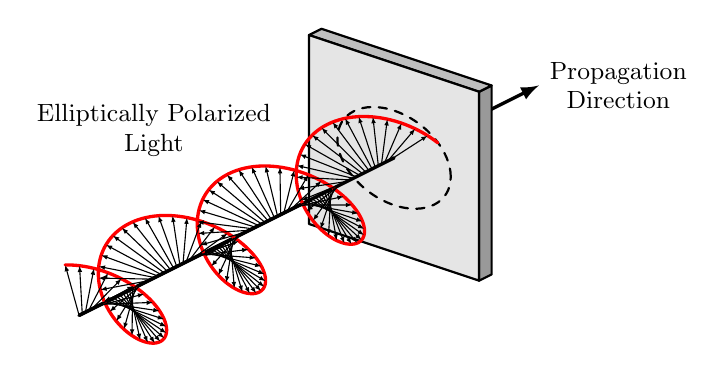
\begin{tikzpicture}[x={(0.8cm, 0.4cm)}, y={(0.9cm, -0.3cm)}, z={(0cm,1cm)}, line cap=round, line join=round]
	
%	% Main Axes
%	\draw[->] (0,0,0) -- (8,0,0) node[right] {$x$};
%	\draw[->] (0,0,0) -- (0,2,0) node[below left] {$y$};
%	\draw[->] (0,0,0) -- (0,0,2) node[above] {$z$};
	
	% Propagation Direction Vector
	\draw[axis] (1,0,0) -- (8.3,0,0) node[right, black] {\small{Propagation}\\[-0.5mm]\small{Direction}};
	
	% Rectangle
	\rect{6}
	
	% Correction so as the Result to Seem 3d
	\draw[very thick] (1,0,0) -- (6,0,0);
	
	% Red Line
	\draw[very thick, red, variable=\t, domain=1:6, samples=300] plot (\t, {0.8*sin(deg(\t*4+90))}, {0.6*cos(deg(\t*4+90))});
	
	% Vectors from Axis to Red Line
	\foreach \i [evaluate={\k = \i*4; \ii = \i;}] in {1,1.05,...,6}
	{
		\draw[vec] (\ii,0,0) -- +(0, {0.8*sin(deg(\k+90))}, {0.6*cos(deg(\k+90))});
	}

	% Nodes
	\node at (5,-2.5) {\small Elliptically Polarized\\[-0.5mm]\small Light};
\end{tikzpicture}

\end{document}